\documentclass[1p]{elsarticle_modified}
%\bibliographystyle{elsarticle-num}

%\usepackage[colorlinks]{hyperref}
%\usepackage{abbrmath_seonhwa} %\Abb, \Ascr, \Acal ,\Abf, \Afrak
\usepackage{amsfonts}
\usepackage{amssymb}
\usepackage{amsmath}
\usepackage{amsthm}
\usepackage{scalefnt}
\usepackage{amsbsy}
\usepackage{kotex}
\usepackage{caption}
\usepackage{subfig}
\usepackage{color}
\usepackage{graphicx}
\usepackage{xcolor} %% white, black, red, green, blue, cyan, magenta, yellow
\usepackage{float}
\usepackage{setspace}
\usepackage{hyperref}

\usepackage{tikz}
\usetikzlibrary{arrows}

\usepackage{multirow}
\usepackage{array} % fixed length table
\usepackage{hhline}

%%%%%%%%%%%%%%%%%%%%%
\makeatletter
\renewcommand*\env@matrix[1][\arraystretch]{%
	\edef\arraystretch{#1}%
	\hskip -\arraycolsep
	\let\@ifnextchar\new@ifnextchar
	\array{*\c@MaxMatrixCols c}}
\makeatother %https://tex.stackexchange.com/questions/14071/how-can-i-increase-the-line-spacing-in-a-matrix
%%%%%%%%%%%%%%%

\usepackage[normalem]{ulem}

\newcommand{\msout}[1]{\ifmmode\text{\sout{\ensuremath{#1}}}\else\sout{#1}\fi}
%SOURCE: \msout is \stkout macro in https://tex.stackexchange.com/questions/20609/strikeout-in-math-mode

\newcommand{\cancel}[1]{
	\ifmmode
	{\color{red}\msout{#1}}
	\else
	{\color{red}\sout{#1}}
	\fi
}

\newcommand{\add}[1]{
	{\color{blue}\uwave{#1}}
}

\newcommand{\replace}[2]{
	\ifmmode
	{\color{red}\msout{#1}}{\color{blue}\uwave{#2}}
	\else
	{\color{red}\sout{#1}}{\color{blue}\uwave{#2}}
	\fi
}

\newcommand{\Sol}{\mathcal{S}} %segment
\newcommand{\D}{D} %diagram
\newcommand{\A}{\mathcal{A}} %arc


%%%%%%%%%%%%%%%%%%%%%%%%%%%%%5 test

\def\sl{\operatorname{\textup{SL}}(2,\Cbb)}
\def\psl{\operatorname{\textup{PSL}}(2,\Cbb)}
\def\quan{\mkern 1mu \triangleright \mkern 1mu}

\theoremstyle{definition}
\newtheorem{thm}{Theorem}[section]
\newtheorem{prop}[thm]{Proposition}
\newtheorem{lem}[thm]{Lemma}
\newtheorem{ques}[thm]{Question}
\newtheorem{cor}[thm]{Corollary}
\newtheorem{defn}[thm]{Definition}
\newtheorem{exam}[thm]{Example}
\newtheorem{rmk}[thm]{Remark}
\newtheorem{alg}[thm]{Algorithm}

\newcommand{\I}{\sqrt{-1}}
\begin{document}

%\begin{frontmatter}
%
%\title{Boundary parabolic representations of knots up to 8 crossings}
%
%%% Group authors per affiliation:
%\author{Yunhi Cho} 
%\address{Department of Mathematics, University of Seoul, Seoul, Korea}
%\ead{yhcho@uos.ac.kr}
%
%
%\author{Seonhwa Kim} %\fnref{s_kim}}
%\address{Center for Geometry and Physics, Institute for Basic Science, Pohang, 37673, Korea}
%\ead{ryeona17@ibs.re.kr}
%
%\author{Hyuk Kim}
%\address{Department of Mathematical Sciences, Seoul National University, Seoul 08826, Korea}
%\ead{hyukkim@snu.ac.kr}
%
%\author{Seokbeom Yoon}
%\address{Department of Mathematical Sciences, Seoul National University, Seoul, 08826,  Korea}
%\ead{sbyoon15@snu.ac.kr}
%
%\begin{abstract}
%We find all boundary parabolic representation of knots up to 8 crossings.
%
%\end{abstract}
%\begin{keyword}
%    \MSC[2010] 57M25 
%\end{keyword}
%
%\end{frontmatter}

%\linenumbers
%\tableofcontents
%
\newcommand\colored[1]{\textcolor{white}{\rule[-0.35ex]{0.8em}{1.4ex}}\kern-0.8em\color{red} #1}%
%\newcommand\colored[1]{\textcolor{white}{ #1}\kern-2.17ex	\textcolor{white}{ #1}\kern-1.81ex	\textcolor{white}{ #1}\kern-2.15ex\color{red}#1	}

{\Large $\underline{12a_{0015}~(K12a_{0015})}$}

\setlength{\tabcolsep}{10pt}
\renewcommand{\arraystretch}{1.6}
\vspace{1cm}\begin{tabular}{m{100pt}>{\centering\arraybackslash}m{274pt}}
\multirow{5}{120pt}{
	\centering
	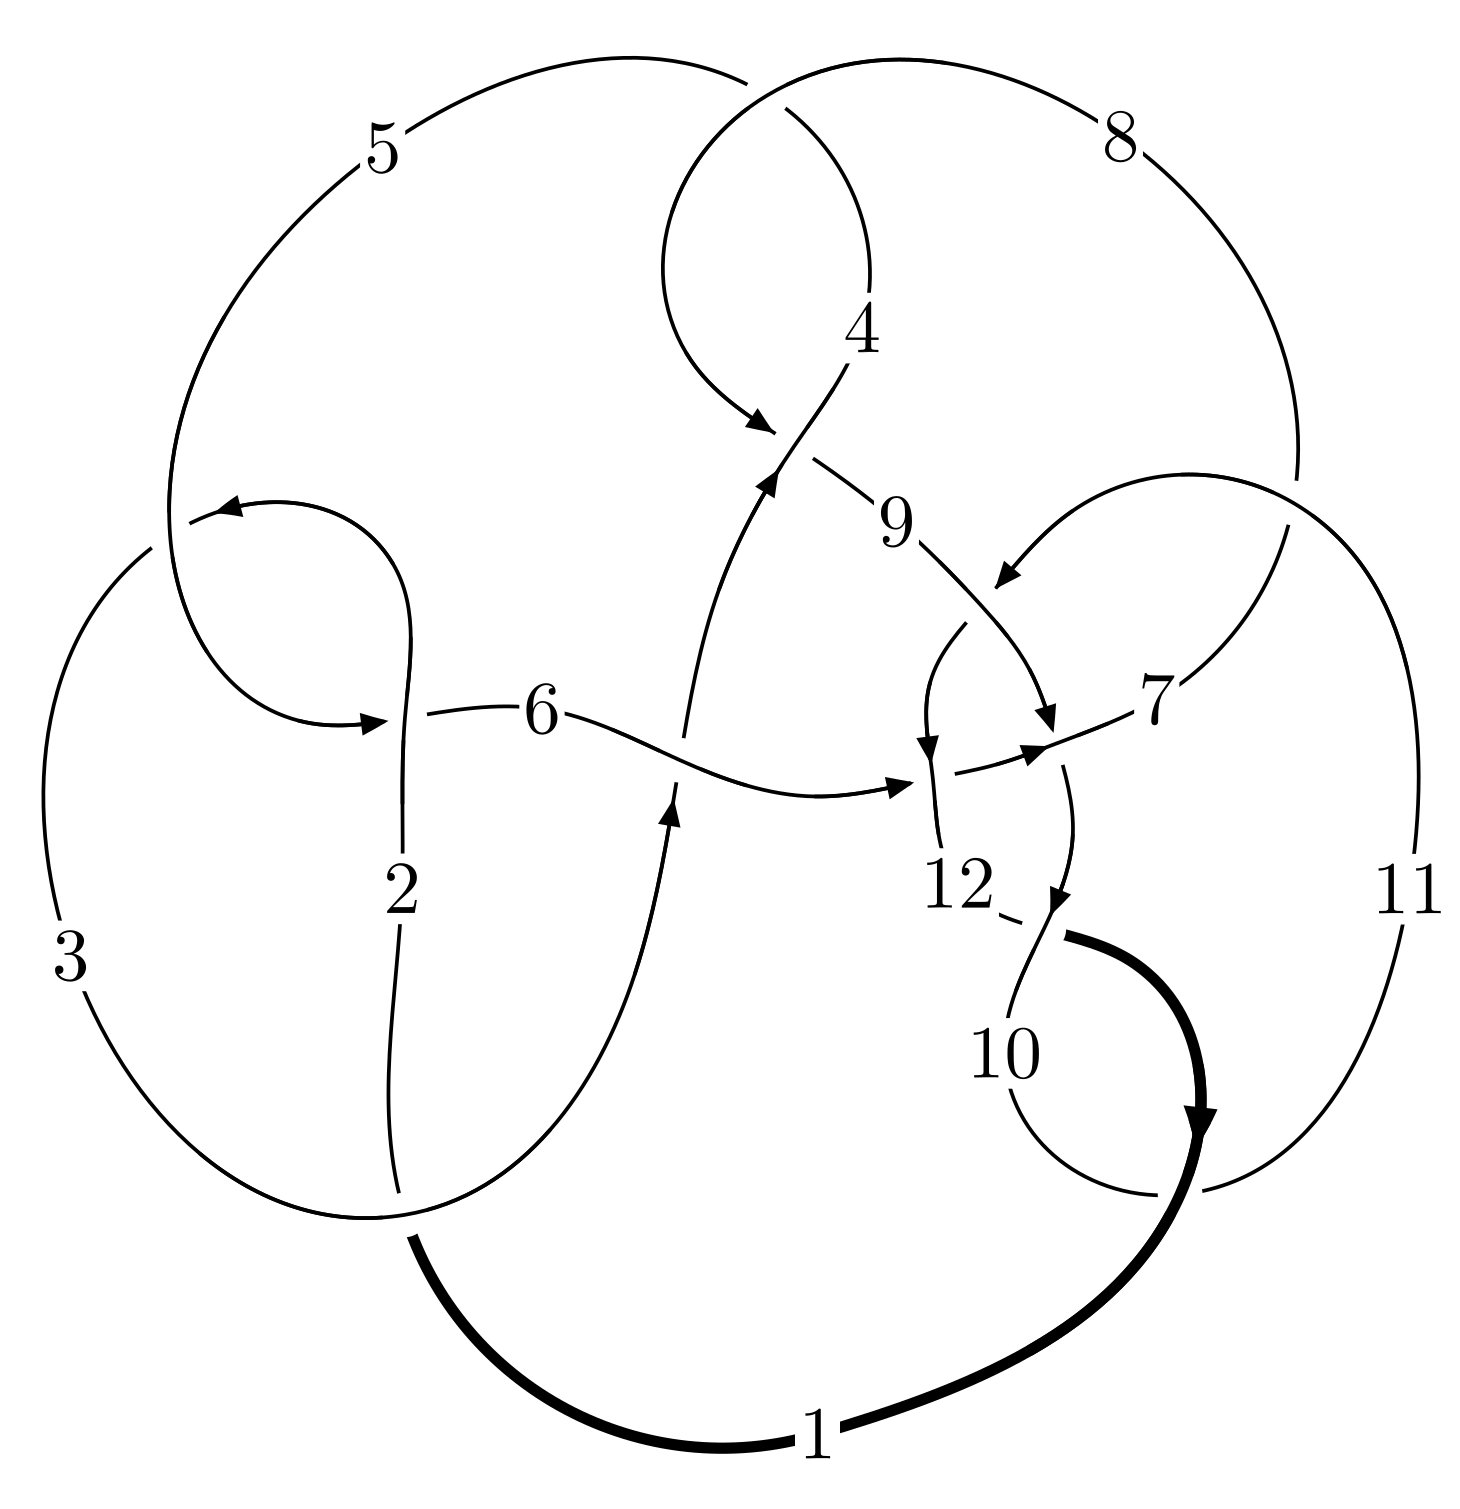
\includegraphics[width=112pt]{../../../GIT/diagram.site/Diagrams/png/816_12a_0015.png}\\
\ \ \ A knot diagram\footnotemark}&
\allowdisplaybreaks
\textbf{Linearized knot diagam} \\
\cline{2-2}
 &
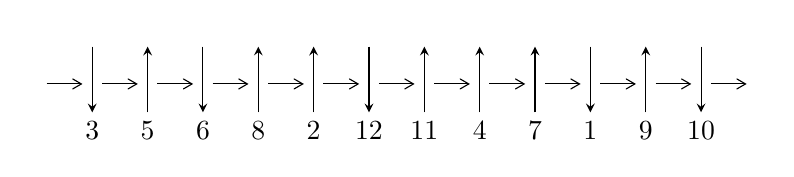
\begin{tikzpicture}[x=20pt, y=17pt]
	% nodes
	\node (C0) at (0, 0) {};
	\node (C1) at (1, 0) {};
	\node (C1U) at (1, +1) {};
	\node (C1D) at (1, -1) {3};

	\node (C2) at (2, 0) {};
	\node (C2U) at (2, +1) {};
	\node (C2D) at (2, -1) {5};

	\node (C3) at (3, 0) {};
	\node (C3U) at (3, +1) {};
	\node (C3D) at (3, -1) {6};

	\node (C4) at (4, 0) {};
	\node (C4U) at (4, +1) {};
	\node (C4D) at (4, -1) {8};

	\node (C5) at (5, 0) {};
	\node (C5U) at (5, +1) {};
	\node (C5D) at (5, -1) {2};

	\node (C6) at (6, 0) {};
	\node (C6U) at (6, +1) {};
	\node (C6D) at (6, -1) {12};

	\node (C7) at (7, 0) {};
	\node (C7U) at (7, +1) {};
	\node (C7D) at (7, -1) {11};

	\node (C8) at (8, 0) {};
	\node (C8U) at (8, +1) {};
	\node (C8D) at (8, -1) {4};

	\node (C9) at (9, 0) {};
	\node (C9U) at (9, +1) {};
	\node (C9D) at (9, -1) {7};

	\node (C10) at (10, 0) {};
	\node (C10U) at (10, +1) {};
	\node (C10D) at (10, -1) {1};

	\node (C11) at (11, 0) {};
	\node (C11U) at (11, +1) {};
	\node (C11D) at (11, -1) {9};

	\node (C12) at (12, 0) {};
	\node (C12U) at (12, +1) {};
	\node (C12D) at (12, -1) {10};
	\node (C13) at (13, 0) {};

	% arrows
	\draw[->,>={angle 60}]
	(C0) edge (C1) (C1) edge (C2) (C2) edge (C3) (C3) edge (C4) (C4) edge (C5) (C5) edge (C6) (C6) edge (C7) (C7) edge (C8) (C8) edge (C9) (C9) edge (C10) (C10) edge (C11) (C11) edge (C12) (C12) edge (C13) ;	\draw[->,>=stealth]
	(C1U) edge (C1D) (C2D) edge (C2U) (C3U) edge (C3D) (C4D) edge (C4U) (C5D) edge (C5U) (C6U) edge (C6D) (C7D) edge (C7U) (C8D) edge (C8U) (C9D) edge (C9U) (C10U) edge (C10D) (C11D) edge (C11U) (C12U) edge (C12D) ;
	\end{tikzpicture} \\
\hhline{~~} \\& 
\textbf{Solving Sequence} \\ \cline{2-2} 
 &
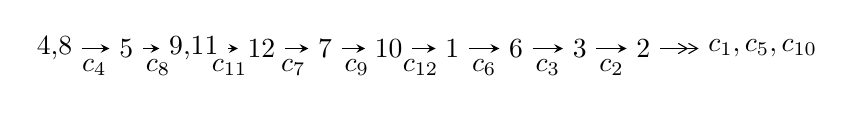
\begin{tikzpicture}[x=23pt, y=7pt]
	% node
	\node (A0) at (-1/8, 0) {4,8};
	\node (A1) at (1, 0) {5};
	\node (A2) at (33/16, 0) {9,11};
	\node (A3) at (25/8, 0) {12};
	\node (A4) at (33/8, 0) {7};
	\node (A5) at (41/8, 0) {10};
	\node (A6) at (49/8, 0) {1};
	\node (A7) at (57/8, 0) {6};
	\node (A8) at (65/8, 0) {3};
	\node (A9) at (73/8, 0) {2};
	\node (C1) at (1/2, -1) {$c_{4}$};
	\node (C2) at (3/2, -1) {$c_{8}$};
	\node (C3) at (21/8, -1) {$c_{11}$};
	\node (C4) at (29/8, -1) {$c_{7}$};
	\node (C5) at (37/8, -1) {$c_{9}$};
	\node (C6) at (45/8, -1) {$c_{12}$};
	\node (C7) at (53/8, -1) {$c_{6}$};
	\node (C8) at (61/8, -1) {$c_{3}$};
	\node (C9) at (69/8, -1) {$c_{2}$};
	\node (A10) at (11, 0) {$c_{1},c_{5},c_{10}$};

	% edge
	\draw[->,>=stealth]	
	(A0) edge (A1) (A1) edge (A2) (A2) edge (A3) (A3) edge (A4) (A4) edge (A5) (A5) edge (A6) (A6) edge (A7) (A7) edge (A8) (A8) edge (A9) ;
	\draw[->>,>={angle 60}]	
	(A9) edge (A10);
\end{tikzpicture} \\ 

\end{tabular} \\

\footnotetext{
The image of knot diagram is generated by the software ``\textbf{Draw programme}" developed by Andrew Bartholomew(\url{http://www.layer8.co.uk/maths/draw/index.htm\#Running-draw}), where we modified some parts for our purpose(\url{https://github.com/CATsTAILs/LinksPainter}).
}\phantom \\ \newline 
\centering \textbf{Ideals for irreducible components\footnotemark of $X_{\text{par}}$} 
 
\begin{align*}
I^u_{1}&=\langle 
2.07638\times10^{604} u^{137}-8.77338\times10^{604} u^{136}+\cdots+8.40968\times10^{606} b-6.86516\times10^{608},\\
\phantom{I^u_{1}}&\phantom{= \langle  }1.65090\times10^{604} u^{137}-8.14368\times10^{604} u^{136}+\cdots+1.68194\times10^{607} a-7.75391\times10^{608},\\
\phantom{I^u_{1}}&\phantom{= \langle  }u^{138}- u^{137}+\cdots+20480 u+4096\rangle \\
\\
I^v_{1}&=\langle 
a,\;963772 v^{11}+658631 v^{10}+\cdots+707733 b+3141326,\\
\phantom{I^v_{1}}&\phantom{= \langle  }v^{12}+v^{11}-4 v^{10}+5 v^9+19 v^8-9 v^7-31 v^6-29 v^5+31 v^4+18 v^3+3 v^2+3 v+1\rangle \\
\end{align*}
\raggedright * 2 irreducible components of $\dim_{\mathbb{C}}=0$, with total 150 representations.\\
\footnotetext{All coefficients of polynomials are rational numbers. But the coefficients are sometimes approximated in decimal forms when there is not enough margin.}
\newpage
\renewcommand{\arraystretch}{1}
\centering \section*{I. $I^u_{1}= \langle 2.08\times10^{604} u^{137}-8.77\times10^{604} u^{136}+\cdots+8.41\times10^{606} b-6.87\times10^{608},\;1.65\times10^{604} u^{137}-8.14\times10^{604} u^{136}+\cdots+1.68\times10^{607} a-7.75\times10^{608},\;u^{138}- u^{137}+\cdots+20480 u+4096 \rangle$}
\flushleft \textbf{(i) Arc colorings}\\
\begin{tabular}{m{7pt} m{180pt} m{7pt} m{180pt} }
\flushright $a_{4}=$&$\begin{pmatrix}1\\0\end{pmatrix}$ \\
\flushright $a_{8}=$&$\begin{pmatrix}0\\u\end{pmatrix}$ \\
\flushright $a_{5}=$&$\begin{pmatrix}1\\- u^2\end{pmatrix}$ \\
\flushright $a_{9}=$&$\begin{pmatrix}u\\u\end{pmatrix}$ \\
\flushright $a_{11}=$&$\begin{pmatrix}-0.000981550 u^{137}+0.00484185 u^{136}+\cdots+217.405 u+46.1011\\-0.00246903 u^{137}+0.0104325 u^{136}+\cdots+395.215 u+81.6340\end{pmatrix}$ \\
\flushright $a_{12}=$&$\begin{pmatrix}-0.000781310 u^{137}+0.00309620 u^{136}+\cdots+139.466 u+29.2946\\-0.00226879 u^{137}+0.00868684 u^{136}+\cdots+317.275 u+64.8275\end{pmatrix}$ \\
\flushright $a_{7}=$&$\begin{pmatrix}0.00204430 u^{137}+0.00306538 u^{136}+\cdots+227.091 u+38.9117\\0.00663207 u^{137}-0.00116817 u^{136}+\cdots+254.146 u+32.6295\end{pmatrix}$ \\
\flushright $a_{10}=$&$\begin{pmatrix}0.00130809 u^{137}-0.00169966 u^{136}+\cdots-15.4882 u-3.73180\\0.000676355 u^{137}+0.00282735 u^{136}+\cdots+176.518 u+33.2890\end{pmatrix}$ \\
\flushright $a_{1}=$&$\begin{pmatrix}0.00439295 u^{137}-0.00147919 u^{136}+\cdots+168.616 u+28.0993\\0.00376122 u^{137}+0.00304781 u^{136}+\cdots+360.623 u+65.1201\end{pmatrix}$ \\
\flushright $a_{6}=$&$\begin{pmatrix}-0.00223744 u^{137}+0.00437981 u^{136}+\cdots+114.339 u+25.0860\\0.00215551 u^{137}+0.00290062 u^{136}+\cdots+282.955 u+53.1853\end{pmatrix}$ \\
\flushright $a_{3}=$&$\begin{pmatrix}0.00294739 u^{137}+0.000658646 u^{136}+\cdots+125.123 u+20.7746\\0.00255322 u^{137}+0.00251675 u^{136}+\cdots+220.759 u+39.9007\end{pmatrix}$ \\
\flushright $a_{2}=$&$\begin{pmatrix}0.00113636 u^{137}-0.000399544 u^{136}+\cdots-9.71148 u-4.35571\\0.00149437 u^{137}+0.00230841 u^{136}+\cdots+154.579 u+28.1483\end{pmatrix}$\\&\end{tabular}
\flushleft \textbf{(ii) Obstruction class $= -1$}\\~\\
\flushleft \textbf{(iii) Cusp Shapes $= -0.0290540 u^{137}+0.0285193 u^{136}+\cdots-46.2850 u+54.5174$}\\~\\
\newpage\renewcommand{\arraystretch}{1}
\flushleft \textbf{(iv) u-Polynomials at the component}\newline \\
\begin{tabular}{m{50pt}|m{274pt}}
Crossings & \hspace{64pt}u-Polynomials at each crossing \\
\hline $$\begin{aligned}c_{1}\end{aligned}$$&$\begin{aligned}
&u^{138}+67 u^{137}+\cdots+33 u+1
\end{aligned}$\\
\hline $$\begin{aligned}c_{2},c_{5}\end{aligned}$$&$\begin{aligned}
&u^{138}+7 u^{137}+\cdots+9 u+1
\end{aligned}$\\
\hline $$\begin{aligned}c_{3}\end{aligned}$$&$\begin{aligned}
&u^{138}-7 u^{137}+\cdots-98472303 u+13657673
\end{aligned}$\\
\hline $$\begin{aligned}c_{4},c_{8}\end{aligned}$$&$\begin{aligned}
&u^{138}- u^{137}+\cdots+20480 u+4096
\end{aligned}$\\
\hline $$\begin{aligned}c_{6}\end{aligned}$$&$\begin{aligned}
&u^{138}-9 u^{137}+\cdots+30021 u-1831
\end{aligned}$\\
\hline $$\begin{aligned}c_{7}\end{aligned}$$&$\begin{aligned}
&u^{138}-3 u^{137}+\cdots+206471 u+14069
\end{aligned}$\\
\hline $$\begin{aligned}c_{9}\end{aligned}$$&$\begin{aligned}
&u^{138}+9 u^{137}+\cdots+3 u+1
\end{aligned}$\\
\hline $$\begin{aligned}c_{10},c_{12}\end{aligned}$$&$\begin{aligned}
&u^{138}-3 u^{137}+\cdots-23 u+1
\end{aligned}$\\
\hline $$\begin{aligned}c_{11}\end{aligned}$$&$\begin{aligned}
&u^{138}+23 u^{137}+\cdots+3 u+1
\end{aligned}$\\
\hline
\end{tabular}\\~\\
\newpage\renewcommand{\arraystretch}{1}
\flushleft \textbf{(v) Riley Polynomials at the component}\newline \\
\begin{tabular}{m{50pt}|m{274pt}}
Crossings & \hspace{64pt}Riley Polynomials at each crossing \\
\hline $$\begin{aligned}c_{1}\end{aligned}$$&$\begin{aligned}
&y^{138}+15 y^{137}+\cdots-35 y+1
\end{aligned}$\\
\hline $$\begin{aligned}c_{2},c_{5}\end{aligned}$$&$\begin{aligned}
&y^{138}+67 y^{137}+\cdots+33 y+1
\end{aligned}$\\
\hline $$\begin{aligned}c_{3}\end{aligned}$$&$\begin{aligned}
&y^{138}-37 y^{137}+\cdots+2159732187820305 y+186532031774929
\end{aligned}$\\
\hline $$\begin{aligned}c_{4},c_{8}\end{aligned}$$&$\begin{aligned}
&y^{138}+65 y^{137}+\cdots+503316480 y+16777216
\end{aligned}$\\
\hline $$\begin{aligned}c_{6}\end{aligned}$$&$\begin{aligned}
&y^{138}-137 y^{137}+\cdots-472810103 y+3352561
\end{aligned}$\\
\hline $$\begin{aligned}c_{7}\end{aligned}$$&$\begin{aligned}
&y^{138}-109 y^{137}+\cdots+23684604833 y+197936761
\end{aligned}$\\
\hline $$\begin{aligned}c_{9}\end{aligned}$$&$\begin{aligned}
&y^{138}+23 y^{137}+\cdots+9 y+1
\end{aligned}$\\
\hline $$\begin{aligned}c_{10},c_{12}\end{aligned}$$&$\begin{aligned}
&y^{138}-89 y^{137}+\cdots-23 y+1
\end{aligned}$\\
\hline $$\begin{aligned}c_{11}\end{aligned}$$&$\begin{aligned}
&y^{138}-9 y^{137}+\cdots-23 y+1
\end{aligned}$\\
\hline
\end{tabular}\\~\\
\newpage\flushleft \textbf{(vi) Complex Volumes and Cusp Shapes}
$$\begin{array}{c|c|c}  
\text{Solutions to }I^u_{1}& \I (\text{vol} + \sqrt{-1}CS) & \text{Cusp shape}\\
 \hline 
\begin{aligned}
u &= -0.225717 + 0.984869 I \\
a &= -0.294640 + 0.216111 I \\
b &= -1.54630 + 0.69058 I\end{aligned}
 & -2.26109 + 1.21839 I & \phantom{-0.000000 } 0 \\ \hline\begin{aligned}
u &= -0.225717 - 0.984869 I \\
a &= -0.294640 - 0.216111 I \\
b &= -1.54630 - 0.69058 I\end{aligned}
 & -2.26109 - 1.21839 I & \phantom{-0.000000 } 0 \\ \hline\begin{aligned}
u &= \phantom{-}0.968613 + 0.291315 I \\
a &= \phantom{-}0.147565 - 0.690953 I \\
b &= \phantom{-}1.43298 + 0.17677 I\end{aligned}
 & -3.85751 - 5.17156 I & \phantom{-0.000000 } 0 \\ \hline\begin{aligned}
u &= \phantom{-}0.968613 - 0.291315 I \\
a &= \phantom{-}0.147565 + 0.690953 I \\
b &= \phantom{-}1.43298 - 0.17677 I\end{aligned}
 & -3.85751 + 5.17156 I & \phantom{-0.000000 } 0 \\ \hline\begin{aligned}
u &= -0.844113 + 0.492611 I \\
a &= -0.358384 - 1.057380 I \\
b &= \phantom{-}0.165311 + 0.318348 I\end{aligned}
 & \phantom{-}2.70862 + 2.80444 I & \phantom{-0.000000 } 0 \\ \hline\begin{aligned}
u &= -0.844113 - 0.492611 I \\
a &= -0.358384 + 1.057380 I \\
b &= \phantom{-}0.165311 - 0.318348 I\end{aligned}
 & \phantom{-}2.70862 - 2.80444 I & \phantom{-0.000000 } 0 \\ \hline\begin{aligned}
u &= -0.495236 + 0.898497 I \\
a &= \phantom{-}1.017350 + 0.325698 I \\
b &= \phantom{-}2.36836 + 0.83423 I\end{aligned}
 & \phantom{-}2.48949 - 5.71532 I & \phantom{-0.000000 } 0 \\ \hline\begin{aligned}
u &= -0.495236 - 0.898497 I \\
a &= \phantom{-}1.017350 - 0.325698 I \\
b &= \phantom{-}2.36836 - 0.83423 I\end{aligned}
 & \phantom{-}2.48949 + 5.71532 I & \phantom{-0.000000 } 0 \\ \hline\begin{aligned}
u &= \phantom{-}0.407051 + 0.951666 I \\
a &= -1.18240 + 1.26696 I \\
b &= -1.79540 + 1.09338 I\end{aligned}
 & -1.49189 + 2.01388 I & \phantom{-0.000000 } 0 \\ \hline\begin{aligned}
u &= \phantom{-}0.407051 - 0.951666 I \\
a &= -1.18240 - 1.26696 I \\
b &= -1.79540 - 1.09338 I\end{aligned}
 & -1.49189 - 2.01388 I & \phantom{-0.000000 } 0\\
 \hline 
 \end{array}$$\newpage$$\begin{array}{c|c|c}  
\text{Solutions to }I^u_{1}& \I (\text{vol} + \sqrt{-1}CS) & \text{Cusp shape}\\
 \hline 
\begin{aligned}
u &= \phantom{-}0.691921 + 0.666142 I \\
a &= -0.667786 + 0.443380 I \\
b &= \phantom{-}0.193633 - 0.004783 I\end{aligned}
 & \phantom{-}1.63530 + 4.17072 I & \phantom{-0.000000 } 0 \\ \hline\begin{aligned}
u &= \phantom{-}0.691921 - 0.666142 I \\
a &= -0.667786 - 0.443380 I \\
b &= \phantom{-}0.193633 + 0.004783 I\end{aligned}
 & \phantom{-}1.63530 - 4.17072 I & \phantom{-0.000000 } 0 \\ \hline\begin{aligned}
u &= \phantom{-}0.647033 + 0.696244 I \\
a &= \phantom{-}0.415181 + 0.391117 I \\
b &= \phantom{-}0.727346 + 0.112079 I\end{aligned}
 & \phantom{-}1.41425 + 1.45110 I & \phantom{-0.000000 } 0 \\ \hline\begin{aligned}
u &= \phantom{-}0.647033 - 0.696244 I \\
a &= \phantom{-}0.415181 - 0.391117 I \\
b &= \phantom{-}0.727346 - 0.112079 I\end{aligned}
 & \phantom{-}1.41425 - 1.45110 I & \phantom{-0.000000 } 0 \\ \hline\begin{aligned}
u &= \phantom{-}0.362183 + 0.876985 I \\
a &= -0.05970 - 1.44009 I \\
b &= -0.197138 + 0.136703 I\end{aligned}
 & \phantom{-}1.44585 + 2.70079 I & \phantom{-0.000000 } 0 \\ \hline\begin{aligned}
u &= \phantom{-}0.362183 - 0.876985 I \\
a &= -0.05970 + 1.44009 I \\
b &= -0.197138 - 0.136703 I\end{aligned}
 & \phantom{-}1.44585 - 2.70079 I & \phantom{-0.000000 } 0 \\ \hline\begin{aligned}
u &= \phantom{-}0.924692 + 0.109605 I \\
a &= \phantom{-}0.345184 + 0.971895 I \\
b &= \phantom{-}1.52213 - 0.03534 I\end{aligned}
 & -4.26855 - 1.64031 I & \phantom{-0.000000 } 0 \\ \hline\begin{aligned}
u &= \phantom{-}0.924692 - 0.109605 I \\
a &= \phantom{-}0.345184 - 0.971895 I \\
b &= \phantom{-}1.52213 + 0.03534 I\end{aligned}
 & -4.26855 + 1.64031 I & \phantom{-0.000000 } 0 \\ \hline\begin{aligned}
u &= -0.790483 + 0.476530 I \\
a &= -0.442068 + 0.500118 I \\
b &= -0.611556 + 0.121924 I\end{aligned}
 & -0.04648 + 3.17550 I & \phantom{-0.000000 } 0 \\ \hline\begin{aligned}
u &= -0.790483 - 0.476530 I \\
a &= -0.442068 - 0.500118 I \\
b &= -0.611556 - 0.121924 I\end{aligned}
 & -0.04648 - 3.17550 I & \phantom{-0.000000 } 0\\
 \hline 
 \end{array}$$\newpage$$\begin{array}{c|c|c}  
\text{Solutions to }I^u_{1}& \I (\text{vol} + \sqrt{-1}CS) & \text{Cusp shape}\\
 \hline 
\begin{aligned}
u &= \phantom{-}0.883665 + 0.175408 I \\
a &= \phantom{-}0.527861 - 0.719630 I \\
b &= -0.049223 + 0.483166 I\end{aligned}
 & -0.821300 - 0.506241 I & \phantom{-0.000000 } 0 \\ \hline\begin{aligned}
u &= \phantom{-}0.883665 - 0.175408 I \\
a &= \phantom{-}0.527861 + 0.719630 I \\
b &= -0.049223 - 0.483166 I\end{aligned}
 & -0.821300 + 0.506241 I & \phantom{-0.000000 } 0 \\ \hline\begin{aligned}
u &= -0.466251 + 0.764985 I \\
a &= \phantom{-}0.742615 + 0.929151 I \\
b &= -0.156769 + 0.062810 I\end{aligned}
 & \phantom{-}0.18427 - 8.79554 I & \phantom{-0.000000 } 0 \\ \hline\begin{aligned}
u &= -0.466251 - 0.764985 I \\
a &= \phantom{-}0.742615 - 0.929151 I \\
b &= -0.156769 - 0.062810 I\end{aligned}
 & \phantom{-}0.18427 + 8.79554 I & \phantom{-0.000000 } 0 \\ \hline\begin{aligned}
u &= \phantom{-}1.000430 + 0.471347 I \\
a &= \phantom{-}0.281303 - 0.942139 I \\
b &= -0.212406 + 0.367643 I\end{aligned}
 & \phantom{-}0.61052 - 7.36350 I & \phantom{-0.000000 } 0 \\ \hline\begin{aligned}
u &= \phantom{-}1.000430 - 0.471347 I \\
a &= \phantom{-}0.281303 + 0.942139 I \\
b &= -0.212406 - 0.367643 I\end{aligned}
 & \phantom{-}0.61052 + 7.36350 I & \phantom{-0.000000 } 0 \\ \hline\begin{aligned}
u &= \phantom{-}0.390996 + 0.800553 I \\
a &= -1.025010 + 0.479217 I \\
b &= -2.38378 + 1.07374 I\end{aligned}
 & \phantom{-}1.65391 + 0.55987 I & \phantom{-0.000000 } 0 \\ \hline\begin{aligned}
u &= \phantom{-}0.390996 - 0.800553 I \\
a &= -1.025010 - 0.479217 I \\
b &= -2.38378 - 1.07374 I\end{aligned}
 & \phantom{-}1.65391 - 0.55987 I & \phantom{-0.000000 } 0 \\ \hline\begin{aligned}
u &= \phantom{-}0.354325 + 1.078600 I \\
a &= \phantom{-}1.182780 - 0.495498 I \\
b &= \phantom{-}2.23291 - 1.06563 I\end{aligned}
 & -2.10779 + 5.70362 I & \phantom{-0.000000 } 0 \\ \hline\begin{aligned}
u &= \phantom{-}0.354325 - 1.078600 I \\
a &= \phantom{-}1.182780 + 0.495498 I \\
b &= \phantom{-}2.23291 + 1.06563 I\end{aligned}
 & -2.10779 - 5.70362 I & \phantom{-0.000000 } 0\\
 \hline 
 \end{array}$$\newpage$$\begin{array}{c|c|c}  
\text{Solutions to }I^u_{1}& \I (\text{vol} + \sqrt{-1}CS) & \text{Cusp shape}\\
 \hline 
\begin{aligned}
u &= \phantom{-}1.13904\phantom{ +0.000000I} \\
a &= \phantom{-}0.622593\phantom{ +0.000000I} \\
b &= \phantom{-}0.160363\phantom{ +0.000000I}\end{aligned}
 & \phantom{-}1.10281\phantom{ +0.000000I} & \phantom{-0.000000 } 0 \\ \hline\begin{aligned}
u &= -0.166480 + 1.130730 I \\
a &= \phantom{-}0.991148 + 0.913261 I \\
b &= \phantom{-}1.60834 + 0.78839 I\end{aligned}
 & -5.25889 + 0.99512 I & \phantom{-0.000000 } 0 \\ \hline\begin{aligned}
u &= -0.166480 - 1.130730 I \\
a &= \phantom{-}0.991148 - 0.913261 I \\
b &= \phantom{-}1.60834 - 0.78839 I\end{aligned}
 & -5.25889 - 0.99512 I & \phantom{-0.000000 } 0 \\ \hline\begin{aligned}
u &= -1.055350 + 0.441739 I \\
a &= \phantom{-}0.456966 + 1.245590 I \\
b &= -0.067158 + 0.137579 I\end{aligned}
 & -1.00538 + 8.27121 I & \phantom{-0.000000 } 0 \\ \hline\begin{aligned}
u &= -1.055350 - 0.441739 I \\
a &= \phantom{-}0.456966 - 1.245590 I \\
b &= -0.067158 - 0.137579 I\end{aligned}
 & -1.00538 - 8.27121 I & \phantom{-0.000000 } 0 \\ \hline\begin{aligned}
u &= -0.805473 + 0.284873 I \\
a &= \phantom{-}3.54683 + 1.54981 I \\
b &= \phantom{-}3.92832 + 1.44251 I\end{aligned}
 & -2.05908 + 3.02563 I & \phantom{-0.000000 } 0 \\ \hline\begin{aligned}
u &= -0.805473 - 0.284873 I \\
a &= \phantom{-}3.54683 - 1.54981 I \\
b &= \phantom{-}3.92832 - 1.44251 I\end{aligned}
 & -2.05908 - 3.02563 I & \phantom{-0.000000 } 0 \\ \hline\begin{aligned}
u &= -0.523047 + 0.667669 I \\
a &= -0.21618 - 1.43239 I \\
b &= \phantom{-}0.160767 + 0.189881 I\end{aligned}
 & \phantom{-}3.16409 + 1.56319 I & \phantom{-0.000000 } 0 \\ \hline\begin{aligned}
u &= -0.523047 - 0.667669 I \\
a &= -0.21618 + 1.43239 I \\
b &= \phantom{-}0.160767 - 0.189881 I\end{aligned}
 & \phantom{-}3.16409 - 1.56319 I & \phantom{-0.000000 } 0 \\ \hline\begin{aligned}
u &= \phantom{-}0.494515 + 1.057540 I \\
a &= \phantom{-}0.96886 - 2.59242 I \\
b &= \phantom{-}1.06381 - 2.11928 I\end{aligned}
 & -2.24796 + 3.24421 I & \phantom{-0.000000 } 0\\
 \hline 
 \end{array}$$\newpage$$\begin{array}{c|c|c}  
\text{Solutions to }I^u_{1}& \I (\text{vol} + \sqrt{-1}CS) & \text{Cusp shape}\\
 \hline 
\begin{aligned}
u &= \phantom{-}0.494515 - 1.057540 I \\
a &= \phantom{-}0.96886 + 2.59242 I \\
b &= \phantom{-}1.06381 + 2.11928 I\end{aligned}
 & -2.24796 - 3.24421 I & \phantom{-0.000000 } 0 \\ \hline\begin{aligned}
u &= -0.147750 + 0.819139 I \\
a &= -0.58094 - 1.46237 I \\
b &= -0.178726 + 0.046191 I\end{aligned}
 & \phantom{-}0.93710 - 3.59535 I & \phantom{-0.000000 } 0 \\ \hline\begin{aligned}
u &= -0.147750 - 0.819139 I \\
a &= -0.58094 + 1.46237 I \\
b &= -0.178726 - 0.046191 I\end{aligned}
 & \phantom{-}0.93710 + 3.59535 I & \phantom{-0.000000 } 0 \\ \hline\begin{aligned}
u &= -0.309016 + 0.768051 I \\
a &= \phantom{-}0.703220 - 0.056139 I \\
b &= \phantom{-}1.58701 - 1.45199 I\end{aligned}
 & -2.00907 - 3.90626 I & \phantom{-0.000000 } 0 \\ \hline\begin{aligned}
u &= -0.309016 - 0.768051 I \\
a &= \phantom{-}0.703220 + 0.056139 I \\
b &= \phantom{-}1.58701 + 1.45199 I\end{aligned}
 & -2.00907 + 3.90626 I & \phantom{-0.000000 } 0 \\ \hline\begin{aligned}
u &= -0.419130 + 1.104740 I \\
a &= -0.741253 + 0.461461 I \\
b &= -1.271310 + 0.295904 I\end{aligned}
 & -4.22588 - 1.00117 I & \phantom{-0.000000 } 0 \\ \hline\begin{aligned}
u &= -0.419130 - 1.104740 I \\
a &= -0.741253 - 0.461461 I \\
b &= -1.271310 - 0.295904 I\end{aligned}
 & -4.22588 + 1.00117 I & \phantom{-0.000000 } 0 \\ \hline\begin{aligned}
u &= -0.403023 + 1.112730 I \\
a &= -0.855650 + 0.551969 I \\
b &= -1.82414 - 0.52868 I\end{aligned}
 & -5.07002 - 1.85762 I & \phantom{-0.000000 } 0 \\ \hline\begin{aligned}
u &= -0.403023 - 1.112730 I \\
a &= -0.855650 - 0.551969 I \\
b &= -1.82414 + 0.52868 I\end{aligned}
 & -5.07002 + 1.85762 I & \phantom{-0.000000 } 0 \\ \hline\begin{aligned}
u &= -0.482224 + 1.095960 I \\
a &= -1.240380 - 0.414603 I \\
b &= -2.33757 - 0.89688 I\end{aligned}
 & -1.36324 - 11.29470 I & \phantom{-0.000000 } 0\\
 \hline 
 \end{array}$$\newpage$$\begin{array}{c|c|c}  
\text{Solutions to }I^u_{1}& \I (\text{vol} + \sqrt{-1}CS) & \text{Cusp shape}\\
 \hline 
\begin{aligned}
u &= -0.482224 - 1.095960 I \\
a &= -1.240380 + 0.414603 I \\
b &= -2.33757 + 0.89688 I\end{aligned}
 & -1.36324 + 11.29470 I & \phantom{-0.000000 } 0 \\ \hline\begin{aligned}
u &= \phantom{-}0.617415 + 1.032780 I \\
a &= \phantom{-}0.678337 + 0.307189 I \\
b &= \phantom{-}1.188460 + 0.067653 I\end{aligned}
 & \phantom{-}0.34659 + 3.64206 I & \phantom{-0.000000 } 0 \\ \hline\begin{aligned}
u &= \phantom{-}0.617415 - 1.032780 I \\
a &= \phantom{-}0.678337 - 0.307189 I \\
b &= \phantom{-}1.188460 - 0.067653 I\end{aligned}
 & \phantom{-}0.34659 - 3.64206 I & \phantom{-0.000000 } 0 \\ \hline\begin{aligned}
u &= -0.299210 + 1.174910 I \\
a &= -0.57189 - 2.80569 I \\
b &= -0.62514 - 2.34158 I\end{aligned}
 & -6.50973 - 0.24697 I & \phantom{-0.000000 } 0 \\ \hline\begin{aligned}
u &= -0.299210 - 1.174910 I \\
a &= -0.57189 + 2.80569 I \\
b &= -0.62514 + 2.34158 I\end{aligned}
 & -6.50973 + 0.24697 I & \phantom{-0.000000 } 0 \\ \hline\begin{aligned}
u &= \phantom{-}0.594539 + 0.516126 I \\
a &= -2.04149 + 2.38783 I \\
b &= -2.48085 + 2.13800 I\end{aligned}
 & -0.564734 + 1.063680 I & -9.1645 - 19.4771 I \\ \hline\begin{aligned}
u &= \phantom{-}0.594539 - 0.516126 I \\
a &= -2.04149 - 2.38783 I \\
b &= -2.48085 - 2.13800 I\end{aligned}
 & -0.564734 - 1.063680 I & -9.1645 + 19.4771 I \\ \hline\begin{aligned}
u &= -0.471282 + 1.118030 I \\
a &= \phantom{-}1.30102 + 1.05181 I \\
b &= \phantom{-}1.89906 + 0.90378 I\end{aligned}
 & -3.90439 - 6.62338 I & \phantom{-0.000000 } 0 \\ \hline\begin{aligned}
u &= -0.471282 - 1.118030 I \\
a &= \phantom{-}1.30102 - 1.05181 I \\
b &= \phantom{-}1.89906 - 0.90378 I\end{aligned}
 & -3.90439 + 6.62338 I & \phantom{-0.000000 } 0 \\ \hline\begin{aligned}
u &= \phantom{-}0.468994 + 0.629619 I \\
a &= \phantom{-}2.43302 - 2.37091 I \\
b &= \phantom{-}2.65913 - 1.95873 I\end{aligned}
 & -0.61751 + 1.70960 I & -9.8208 + 17.9498 I\\
 \hline 
 \end{array}$$\newpage$$\begin{array}{c|c|c}  
\text{Solutions to }I^u_{1}& \I (\text{vol} + \sqrt{-1}CS) & \text{Cusp shape}\\
 \hline 
\begin{aligned}
u &= \phantom{-}0.468994 - 0.629619 I \\
a &= \phantom{-}2.43302 + 2.37091 I \\
b &= \phantom{-}2.65913 + 1.95873 I\end{aligned}
 & -0.61751 - 1.70960 I & -9.8208 - 17.9498 I \\ \hline\begin{aligned}
u &= \phantom{-}0.382806 + 1.155410 I \\
a &= \phantom{-}0.359131 + 0.027006 I \\
b &= \phantom{-}1.60372 + 0.55083 I\end{aligned}
 & -4.91525 + 3.17082 I & \phantom{-0.000000 } 0 \\ \hline\begin{aligned}
u &= \phantom{-}0.382806 - 1.155410 I \\
a &= \phantom{-}0.359131 - 0.027006 I \\
b &= \phantom{-}1.60372 - 0.55083 I\end{aligned}
 & -4.91525 - 3.17082 I & \phantom{-0.000000 } 0 \\ \hline\begin{aligned}
u &= \phantom{-}0.080035 + 1.216100 I \\
a &= \phantom{-}0.526288 + 0.157565 I \\
b &= \phantom{-}1.74683 + 0.65547 I\end{aligned}
 & -5.86217 - 4.68661 I & \phantom{-0.000000 } 0 \\ \hline\begin{aligned}
u &= \phantom{-}0.080035 - 1.216100 I \\
a &= \phantom{-}0.526288 - 0.157565 I \\
b &= \phantom{-}1.74683 - 0.65547 I\end{aligned}
 & -5.86217 + 4.68661 I & \phantom{-0.000000 } 0 \\ \hline\begin{aligned}
u &= \phantom{-}1.204080 + 0.239536 I \\
a &= -0.459385 + 1.051260 I \\
b &= \phantom{-}0.090805 + 0.133302 I\end{aligned}
 & -5.12215 - 5.13211 I & \phantom{-0.000000 } 0 \\ \hline\begin{aligned}
u &= \phantom{-}1.204080 - 0.239536 I \\
a &= -0.459385 - 1.051260 I \\
b &= \phantom{-}0.090805 - 0.133302 I\end{aligned}
 & -5.12215 + 5.13211 I & \phantom{-0.000000 } 0 \\ \hline\begin{aligned}
u &= -0.514859 + 1.134730 I \\
a &= \phantom{-}0.541995 + 0.245560 I \\
b &= \phantom{-}1.32232 - 0.99331 I\end{aligned}
 & -4.22507 - 5.81215 I & \phantom{-0.000000 } 0 \\ \hline\begin{aligned}
u &= -0.514859 - 1.134730 I \\
a &= \phantom{-}0.541995 - 0.245560 I \\
b &= \phantom{-}1.32232 + 0.99331 I\end{aligned}
 & -4.22507 + 5.81215 I & \phantom{-0.000000 } 0 \\ \hline\begin{aligned}
u &= -0.752443 + 0.039638 I \\
a &= -0.852096 + 0.385900 I \\
b &= -0.613279 - 0.275254 I\end{aligned}
 & -1.00356 - 2.77254 I & \phantom{-}0.77684 + 5.56890 I\\
 \hline 
 \end{array}$$\newpage$$\begin{array}{c|c|c}  
\text{Solutions to }I^u_{1}& \I (\text{vol} + \sqrt{-1}CS) & \text{Cusp shape}\\
 \hline 
\begin{aligned}
u &= -0.752443 - 0.039638 I \\
a &= -0.852096 - 0.385900 I \\
b &= -0.613279 + 0.275254 I\end{aligned}
 & -1.00356 + 2.77254 I & \phantom{-}0.77684 - 5.56890 I \\ \hline\begin{aligned}
u &= -0.536143 + 0.485236 I \\
a &= \phantom{-}0.51276 + 1.88327 I \\
b &= -0.0175137 + 0.1051560 I\end{aligned}
 & \phantom{-}0.61191 + 7.14983 I & \phantom{-}3.75978 - 1.57652 I \\ \hline\begin{aligned}
u &= -0.536143 - 0.485236 I \\
a &= \phantom{-}0.51276 - 1.88327 I \\
b &= -0.0175137 - 0.1051560 I\end{aligned}
 & \phantom{-}0.61191 - 7.14983 I & \phantom{-}3.75978 + 1.57652 I \\ \hline\begin{aligned}
u &= \phantom{-}0.722812\phantom{ +0.000000I} \\
a &= \phantom{-}1.01964\phantom{ +0.000000I} \\
b &= \phantom{-}0.245406\phantom{ +0.000000I}\end{aligned}
 & \phantom{-}1.24576\phantom{ +0.000000I} & \phantom{-}9.34870\phantom{ +0.000000I} \\ \hline\begin{aligned}
u &= -0.633518 + 0.347110 I \\
a &= \phantom{-}0.253544 - 0.635653 I \\
b &= -1.255390 + 0.218624 I\end{aligned}
 & -1.79923 + 1.22022 I & -1.34511 - 3.56182 I \\ \hline\begin{aligned}
u &= -0.633518 - 0.347110 I \\
a &= \phantom{-}0.253544 + 0.635653 I \\
b &= -1.255390 - 0.218624 I\end{aligned}
 & -1.79923 - 1.22022 I & -1.34511 + 3.56182 I \\ \hline\begin{aligned}
u &= \phantom{-}0.229996 + 1.259400 I \\
a &= -0.198398 + 0.489472 I \\
b &= -0.374227 + 0.829231 I\end{aligned}
 & \phantom{-}0.42778 + 2.94009 I & \phantom{-0.000000 } 0 \\ \hline\begin{aligned}
u &= \phantom{-}0.229996 - 1.259400 I \\
a &= -0.198398 - 0.489472 I \\
b &= -0.374227 - 0.829231 I\end{aligned}
 & \phantom{-}0.42778 - 2.94009 I & \phantom{-0.000000 } 0 \\ \hline\begin{aligned}
u &= \phantom{-}0.237164 + 1.259150 I \\
a &= \phantom{-}0.793025 + 0.477523 I \\
b &= \phantom{-}1.72121 - 0.62807 I\end{aligned}
 & -9.23975 - 1.47869 I & \phantom{-0.000000 } 0 \\ \hline\begin{aligned}
u &= \phantom{-}0.237164 - 1.259150 I \\
a &= \phantom{-}0.793025 - 0.477523 I \\
b &= \phantom{-}1.72121 + 0.62807 I\end{aligned}
 & -9.23975 + 1.47869 I & \phantom{-0.000000 } 0\\
 \hline 
 \end{array}$$\newpage$$\begin{array}{c|c|c}  
\text{Solutions to }I^u_{1}& \I (\text{vol} + \sqrt{-1}CS) & \text{Cusp shape}\\
 \hline 
\begin{aligned}
u &= -0.625704 + 1.124680 I \\
a &= \phantom{-}0.957652 + 0.155716 I \\
b &= \phantom{-}2.25228 + 0.59171 I\end{aligned}
 & \phantom{-}0.72901 - 8.31835 I & \phantom{-0.000000 } 0 \\ \hline\begin{aligned}
u &= -0.625704 - 1.124680 I \\
a &= \phantom{-}0.957652 - 0.155716 I \\
b &= \phantom{-}2.25228 - 0.59171 I\end{aligned}
 & \phantom{-}0.72901 + 8.31835 I & \phantom{-0.000000 } 0 \\ \hline\begin{aligned}
u &= \phantom{-}1.179740 + 0.520421 I \\
a &= -0.361647 + 1.213850 I \\
b &= \phantom{-}0.071610 + 0.151034 I\end{aligned}
 & -3.53057 - 13.07050 I & \phantom{-0.000000 } 0 \\ \hline\begin{aligned}
u &= \phantom{-}1.179740 - 0.520421 I \\
a &= -0.361647 - 1.213850 I \\
b &= \phantom{-}0.071610 - 0.151034 I\end{aligned}
 & -3.53057 + 13.07050 I & \phantom{-0.000000 } 0 \\ \hline\begin{aligned}
u &= \phantom{-}0.185406 + 0.682883 I \\
a &= \phantom{-}0.27266 + 1.97980 I \\
b &= -0.0381996 + 0.1034590 I\end{aligned}
 & -0.44372 - 3.17076 I & -5.30905 - 2.16030 I \\ \hline\begin{aligned}
u &= \phantom{-}0.185406 - 0.682883 I \\
a &= \phantom{-}0.27266 - 1.97980 I \\
b &= -0.0381996 - 0.1034590 I\end{aligned}
 & -0.44372 + 3.17076 I & -5.30905 + 2.16030 I \\ \hline\begin{aligned}
u &= -0.557227 + 1.166990 I \\
a &= -0.81226 - 2.43716 I \\
b &= -0.89747 - 1.94437 I\end{aligned}
 & -4.70709 - 8.12492 I & \phantom{-0.000000 } 0 \\ \hline\begin{aligned}
u &= -0.557227 - 1.166990 I \\
a &= -0.81226 + 2.43716 I \\
b &= -0.89747 + 1.94437 I\end{aligned}
 & -4.70709 + 8.12492 I & \phantom{-0.000000 } 0 \\ \hline\begin{aligned}
u &= \phantom{-}0.484539 + 1.201990 I \\
a &= -0.873032 + 0.170491 I \\
b &= -2.13899 + 0.63134 I\end{aligned}
 & -4.09738 + 5.40863 I & \phantom{-0.000000 } 0 \\ \hline\begin{aligned}
u &= \phantom{-}0.484539 - 1.201990 I \\
a &= -0.873032 - 0.170491 I \\
b &= -2.13899 - 0.63134 I\end{aligned}
 & -4.09738 - 5.40863 I & \phantom{-0.000000 } 0\\
 \hline 
 \end{array}$$\newpage$$\begin{array}{c|c|c}  
\text{Solutions to }I^u_{1}& \I (\text{vol} + \sqrt{-1}CS) & \text{Cusp shape}\\
 \hline 
\begin{aligned}
u &= -0.652158 + 1.121780 I \\
a &= -0.753877 + 0.285874 I \\
b &= -1.301380 + 0.047036 I\end{aligned}
 & -1.92373 - 8.69899 I & \phantom{-0.000000 } 0 \\ \hline\begin{aligned}
u &= -0.652158 - 1.121780 I \\
a &= -0.753877 - 0.285874 I \\
b &= -1.301380 - 0.047036 I\end{aligned}
 & -1.92373 + 8.69899 I & \phantom{-0.000000 } 0 \\ \hline\begin{aligned}
u &= \phantom{-}0.354774 + 1.248840 I \\
a &= -0.616679 + 0.303202 I \\
b &= -1.43627 - 0.89821 I\end{aligned}
 & -8.72518 + 2.65013 I & \phantom{-0.000000 } 0 \\ \hline\begin{aligned}
u &= \phantom{-}0.354774 - 1.248840 I \\
a &= -0.616679 - 0.303202 I \\
b &= -1.43627 + 0.89821 I\end{aligned}
 & -8.72518 - 2.65013 I & \phantom{-0.000000 } 0 \\ \hline\begin{aligned}
u &= \phantom{-}0.456208 + 0.530857 I \\
a &= \phantom{-}1.13919 - 1.09802 I \\
b &= \phantom{-}0.157090 - 0.007597 I\end{aligned}
 & \phantom{-}2.30178 - 0.05398 I & \phantom{-}5.52630 - 2.50446 I \\ \hline\begin{aligned}
u &= \phantom{-}0.456208 - 0.530857 I \\
a &= \phantom{-}1.13919 + 1.09802 I \\
b &= \phantom{-}0.157090 + 0.007597 I\end{aligned}
 & \phantom{-}2.30178 + 0.05398 I & \phantom{-}5.52630 + 2.50446 I \\ \hline\begin{aligned}
u &= \phantom{-}0.969289 + 0.894952 I \\
a &= -0.1042660 - 0.0526307 I \\
b &= \phantom{-}0.190558 - 0.272536 I\end{aligned}
 & \phantom{-}1.00721 + 1.59954 I & \phantom{-0.000000 } 0 \\ \hline\begin{aligned}
u &= \phantom{-}0.969289 - 0.894952 I \\
a &= -0.1042660 + 0.0526307 I \\
b &= \phantom{-}0.190558 + 0.272536 I\end{aligned}
 & \phantom{-}1.00721 - 1.59954 I & \phantom{-0.000000 } 0 \\ \hline\begin{aligned}
u &= \phantom{-}0.499313 + 1.221980 I \\
a &= \phantom{-}0.800563 + 0.576581 I \\
b &= \phantom{-}1.75153 - 0.48262 I\end{aligned}
 & -7.72780 + 6.66125 I & \phantom{-0.000000 } 0 \\ \hline\begin{aligned}
u &= \phantom{-}0.499313 - 1.221980 I \\
a &= \phantom{-}0.800563 - 0.576581 I \\
b &= \phantom{-}1.75153 + 0.48262 I\end{aligned}
 & -7.72780 - 6.66125 I & \phantom{-0.000000 } 0\\
 \hline 
 \end{array}$$\newpage$$\begin{array}{c|c|c}  
\text{Solutions to }I^u_{1}& \I (\text{vol} + \sqrt{-1}CS) & \text{Cusp shape}\\
 \hline 
\begin{aligned}
u &= -0.027575 + 0.669982 I \\
a &= -0.131081 + 0.975115 I \\
b &= -0.33991 + 1.63785 I\end{aligned}
 & \phantom{-}0.77901 + 2.40486 I & \phantom{-}0.57490 - 3.33955 I \\ \hline\begin{aligned}
u &= -0.027575 - 0.669982 I \\
a &= -0.131081 - 0.975115 I \\
b &= -0.33991 - 1.63785 I\end{aligned}
 & \phantom{-}0.77901 - 2.40486 I & \phantom{-}0.57490 + 3.33955 I \\ \hline\begin{aligned}
u &= -1.239130 + 0.488019 I \\
a &= \phantom{-}0.294086 - 0.385560 I \\
b &= -0.134296 - 0.114140 I\end{aligned}
 & -4.27455 - 4.31705 I & \phantom{-0.000000 } 0 \\ \hline\begin{aligned}
u &= -1.239130 - 0.488019 I \\
a &= \phantom{-}0.294086 + 0.385560 I \\
b &= -0.134296 + 0.114140 I\end{aligned}
 & -4.27455 + 4.31705 I & \phantom{-0.000000 } 0 \\ \hline\begin{aligned}
u &= -0.760986 + 1.097480 I \\
a &= \phantom{-}0.114324 - 0.213713 I \\
b &= \phantom{-}0.064421 - 0.580905 I\end{aligned}
 & -0.61746 + 4.04978 I & \phantom{-0.000000 } 0 \\ \hline\begin{aligned}
u &= -0.760986 - 1.097480 I \\
a &= \phantom{-}0.114324 + 0.213713 I \\
b &= \phantom{-}0.064421 + 0.580905 I\end{aligned}
 & -0.61746 - 4.04978 I & \phantom{-0.000000 } 0 \\ \hline\begin{aligned}
u &= -0.533533 + 0.393622 I \\
a &= -0.97725 + 1.40364 I \\
b &= -1.94209 + 0.34526 I\end{aligned}
 & -2.78368 - 1.46397 I & -3.71074 + 3.08918 I \\ \hline\begin{aligned}
u &= -0.533533 - 0.393622 I \\
a &= -0.97725 - 1.40364 I \\
b &= -1.94209 - 0.34526 I\end{aligned}
 & -2.78368 + 1.46397 I & -3.71074 - 3.08918 I \\ \hline\begin{aligned}
u &= \phantom{-}0.047521 + 0.644878 I \\
a &= -1.179240 - 0.068407 I \\
b &= -2.32332 - 1.43336 I\end{aligned}
 & -2.35739 - 0.94653 I & -10.41057 - 1.05373 I \\ \hline\begin{aligned}
u &= \phantom{-}0.047521 - 0.644878 I \\
a &= -1.179240 + 0.068407 I \\
b &= -2.32332 + 1.43336 I\end{aligned}
 & -2.35739 + 0.94653 I & -10.41057 + 1.05373 I\\
 \hline 
 \end{array}$$\newpage$$\begin{array}{c|c|c}  
\text{Solutions to }I^u_{1}& \I (\text{vol} + \sqrt{-1}CS) & \text{Cusp shape}\\
 \hline 
\begin{aligned}
u &= \phantom{-}0.589342 + 1.220770 I \\
a &= -0.514128 + 0.291135 I \\
b &= -1.27522 - 0.92426 I\end{aligned}
 & -6.77899 + 10.82090 I & \phantom{-0.000000 } 0 \\ \hline\begin{aligned}
u &= \phantom{-}0.589342 - 1.220770 I \\
a &= -0.514128 - 0.291135 I \\
b &= -1.27522 + 0.92426 I\end{aligned}
 & -6.77899 - 10.82090 I & \phantom{-0.000000 } 0 \\ \hline\begin{aligned}
u &= \phantom{-}0.678071 + 1.188740 I \\
a &= -0.952054 + 0.115631 I \\
b &= -2.23325 + 0.53630 I\end{aligned}
 & -1.67408 + 13.49120 I & \phantom{-0.000000 } 0 \\ \hline\begin{aligned}
u &= \phantom{-}0.678071 - 1.188740 I \\
a &= -0.952054 - 0.115631 I \\
b &= -2.23325 - 0.53630 I\end{aligned}
 & -1.67408 - 13.49120 I & \phantom{-0.000000 } 0 \\ \hline\begin{aligned}
u &= -0.699582 + 1.215180 I \\
a &= -1.250860 - 0.275217 I \\
b &= -2.33543 - 0.61493 I\end{aligned}
 & -3.4406 - 14.6175 I & \phantom{-0.000000 } 0 \\ \hline\begin{aligned}
u &= -0.699582 - 1.215180 I \\
a &= -1.250860 + 0.275217 I \\
b &= -2.33543 + 0.61493 I\end{aligned}
 & -3.4406 + 14.6175 I & \phantom{-0.000000 } 0 \\ \hline\begin{aligned}
u &= -0.06214 + 1.41839 I \\
a &= \phantom{-}0.821700 - 0.319634 I \\
b &= \phantom{-}1.51310 - 0.76091 I\end{aligned}
 & -7.96952 + 4.57151 I & \phantom{-0.000000 } 0 \\ \hline\begin{aligned}
u &= -0.06214 - 1.41839 I \\
a &= \phantom{-}0.821700 + 0.319634 I \\
b &= \phantom{-}1.51310 + 0.76091 I\end{aligned}
 & -7.96952 - 4.57151 I & \phantom{-0.000000 } 0 \\ \hline\begin{aligned}
u &= -0.447357 + 0.348451 I \\
a &= -3.00586 - 0.37306 I \\
b &= -3.58489 + 0.07302 I\end{aligned}
 & -1.48464 + 2.67615 I & -11.3832 + 12.0268 I \\ \hline\begin{aligned}
u &= -0.447357 - 0.348451 I \\
a &= -3.00586 + 0.37306 I \\
b &= -3.58489 - 0.07302 I\end{aligned}
 & -1.48464 - 2.67615 I & -11.3832 - 12.0268 I\\
 \hline 
 \end{array}$$\newpage$$\begin{array}{c|c|c}  
\text{Solutions to }I^u_{1}& \I (\text{vol} + \sqrt{-1}CS) & \text{Cusp shape}\\
 \hline 
\begin{aligned}
u &= -1.36012 + 0.45602 I \\
a &= -0.330074 - 0.370600 I \\
b &= -0.146651 - 0.049871 I\end{aligned}
 & -2.10145 + 4.63629 I & \phantom{-0.000000 } 0 \\ \hline\begin{aligned}
u &= -1.36012 - 0.45602 I \\
a &= -0.330074 + 0.370600 I \\
b &= -0.146651 + 0.049871 I\end{aligned}
 & -2.10145 - 4.63629 I & \phantom{-0.000000 } 0 \\ \hline\begin{aligned}
u &= \phantom{-}0.60934 + 1.31602 I \\
a &= \phantom{-}1.191370 - 0.282012 I \\
b &= \phantom{-}2.21784 - 0.64053 I\end{aligned}
 & -8.6772 + 11.5041 I & \phantom{-0.000000 } 0 \\ \hline\begin{aligned}
u &= \phantom{-}0.60934 - 1.31602 I \\
a &= \phantom{-}1.191370 + 0.282012 I \\
b &= \phantom{-}2.21784 + 0.64053 I\end{aligned}
 & -8.6772 - 11.5041 I & \phantom{-0.000000 } 0 \\ \hline\begin{aligned}
u &= \phantom{-}0.69110 + 1.28047 I \\
a &= -0.618692 + 0.364479 I \\
b &= -1.177280 + 0.552949 I\end{aligned}
 & -2.30827 + 6.50477 I & \phantom{-0.000000 } 0 \\ \hline\begin{aligned}
u &= \phantom{-}0.69110 - 1.28047 I \\
a &= -0.618692 - 0.364479 I \\
b &= -1.177280 - 0.552949 I\end{aligned}
 & -2.30827 - 6.50477 I & \phantom{-0.000000 } 0 \\ \hline\begin{aligned}
u &= \phantom{-}0.76319 + 1.24643 I \\
a &= \phantom{-}1.251390 - 0.245316 I \\
b &= \phantom{-}2.33016 - 0.55434 I\end{aligned}
 & -5.8957 + 20.0114 I & \phantom{-0.000000 } 0 \\ \hline\begin{aligned}
u &= \phantom{-}0.76319 - 1.24643 I \\
a &= \phantom{-}1.251390 + 0.245316 I \\
b &= \phantom{-}2.33016 + 0.55434 I\end{aligned}
 & -5.8957 - 20.0114 I & \phantom{-0.000000 } 0 \\ \hline\begin{aligned}
u &= -0.76896 + 1.29555 I \\
a &= \phantom{-}0.676542 + 0.349738 I \\
b &= \phantom{-}1.289450 + 0.515918 I\end{aligned}
 & -4.86223 - 11.95560 I & \phantom{-0.000000 } 0 \\ \hline\begin{aligned}
u &= -0.76896 - 1.29555 I \\
a &= \phantom{-}0.676542 - 0.349738 I \\
b &= \phantom{-}1.289450 - 0.515918 I\end{aligned}
 & -4.86223 + 11.95560 I & \phantom{-0.000000 } 0\\
 \hline 
 \end{array}$$\newpage$$\begin{array}{c|c|c}  
\text{Solutions to }I^u_{1}& \I (\text{vol} + \sqrt{-1}CS) & \text{Cusp shape}\\
 \hline 
\begin{aligned}
u &= -0.07354 + 1.51167 I \\
a &= -0.916297 - 0.278761 I \\
b &= -1.68989 - 0.67622 I\end{aligned}
 & -11.8703 - 9.0599 I & \phantom{-0.000000 } 0 \\ \hline\begin{aligned}
u &= -0.07354 - 1.51167 I \\
a &= -0.916297 + 0.278761 I \\
b &= -1.68989 + 0.67622 I\end{aligned}
 & -11.8703 + 9.0599 I & \phantom{-0.000000 } 0 \\ \hline\begin{aligned}
u &= -0.269804 + 0.381004 I \\
a &= \phantom{-}1.069040 + 0.014526 I \\
b &= -0.926287 + 0.440409 I\end{aligned}
 & -1.85090 + 1.10618 I & -2.51777 - 1.83567 I \\ \hline\begin{aligned}
u &= -0.269804 - 0.381004 I \\
a &= \phantom{-}1.069040 - 0.014526 I \\
b &= -0.926287 - 0.440409 I\end{aligned}
 & -1.85090 - 1.10618 I & -2.51777 + 1.83567 I \\ \hline\begin{aligned}
u &= \phantom{-}0.17686 + 1.52587 I \\
a &= -0.777083 - 0.221638 I \\
b &= -1.42378 - 0.57653 I\end{aligned}
 & -11.67560 + 0.10597 I & \phantom{-0.000000 } 0 \\ \hline\begin{aligned}
u &= \phantom{-}0.17686 - 1.52587 I \\
a &= -0.777083 + 0.221638 I \\
b &= -1.42378 + 0.57653 I\end{aligned}
 & -11.67560 - 0.10597 I & \phantom{-0.000000 } 0 \\ \hline\begin{aligned}
u &= -0.63750 + 1.40717 I \\
a &= \phantom{-}0.576430 + 0.245891 I \\
b &= \phantom{-}1.079120 + 0.326947 I\end{aligned}
 & -7.63817 - 3.16727 I & \phantom{-0.000000 } 0 \\ \hline\begin{aligned}
u &= -0.63750 - 1.40717 I \\
a &= \phantom{-}0.576430 - 0.245891 I \\
b &= \phantom{-}1.079120 - 0.326947 I\end{aligned}
 & -7.63817 + 3.16727 I & \phantom{-0.000000 } 0\\
 \hline 
 \end{array}$$\newpage\newpage\renewcommand{\arraystretch}{1}
\centering \section*{II. $I^v_{1}= \langle a,\;9.64\times10^{5} v^{11}+6.59\times10^{5} v^{10}+\cdots+7.08\times10^{5} b+3.14\times10^{6},\;v^{12}+v^{11}+\cdots+3 v+1 \rangle$}
\flushleft \textbf{(i) Arc colorings}\\
\begin{tabular}{m{7pt} m{180pt} m{7pt} m{180pt} }
\flushright $a_{4}=$&$\begin{pmatrix}1\\0\end{pmatrix}$ \\
\flushright $a_{8}=$&$\begin{pmatrix}v\\0\end{pmatrix}$ \\
\flushright $a_{5}=$&$\begin{pmatrix}1\\0\end{pmatrix}$ \\
\flushright $a_{9}=$&$\begin{pmatrix}v\\0\end{pmatrix}$ \\
\flushright $a_{11}=$&$\begin{pmatrix}0\\-1.36177 v^{11}-0.930621 v^{10}+\cdots-5.08294 v-4.43857\end{pmatrix}$ \\
\flushright $a_{12}=$&$\begin{pmatrix}-0.222666 v^{11}-0.152658 v^{10}+\cdots+0.0683153 v-0.431153\\-1.36177 v^{11}-0.930621 v^{10}+\cdots-5.08294 v-4.43857\end{pmatrix}$ \\
\flushright $a_{7}=$&$\begin{pmatrix}v\\-0.546453 v^{11}-0.201388 v^{10}+\cdots-2.43405 v-1.91940\end{pmatrix}$ \\
\flushright $a_{10}=$&$\begin{pmatrix}0.181358 v^{11}+0.113940 v^{10}+\cdots+1.48874 v+0.345065\\-0.678951 v^{11}-0.501804 v^{10}+\cdots-2.40704 v-2.15346\end{pmatrix}$ \\
\flushright $a_{1}=$&$\begin{pmatrix}-0.306346 v^{11}-0.227326 v^{10}+\cdots-1.34123 v-0.522212\\-0.678951 v^{11}-0.501804 v^{10}+\cdots-2.40704 v-2.15346\end{pmatrix}$ \\
\flushright $a_{6}=$&$\begin{pmatrix}0.306346 v^{11}+0.227326 v^{10}+\cdots+1.34123 v+0.522212\\0.678951 v^{11}+0.501804 v^{10}+\cdots+2.40704 v+2.15346\end{pmatrix}$ \\
\flushright $a_{3}=$&$\begin{pmatrix}0.0350655 v^{11}-0.0129173 v^{10}+\cdots-0.00328231 v+1.62035\\-0.678951 v^{11}-0.501804 v^{10}+\cdots-2.40704 v-1.15346\end{pmatrix}$ \\
\flushright $a_{2}=$&$\begin{pmatrix}0.714016 v^{11}+0.488886 v^{10}+\cdots+2.40376 v+2.77380\\-0.678951 v^{11}-0.501804 v^{10}+\cdots-2.40704 v-1.15346\end{pmatrix}$\\&\end{tabular}
\flushleft \textbf{(ii) Obstruction class $= 1$}\\~\\
\flushleft \textbf{(iii) Cusp Shapes $= \frac{821}{10257} v^{11}+\frac{8666}{235911} v^{10}+\cdots+\frac{189289}{10257} v+\frac{16124}{235911}$}\\~\\
\newpage\renewcommand{\arraystretch}{1}
\flushleft \textbf{(iv) u-Polynomials at the component}\newline \\
\begin{tabular}{m{50pt}|m{274pt}}
Crossings & \hspace{64pt}u-Polynomials at each crossing \\
\hline $$\begin{aligned}c_{1},c_{3},c_{5}\end{aligned}$$&$\begin{aligned}
&(u^2- u+1)^6
\end{aligned}$\\
\hline $$\begin{aligned}c_{2}\end{aligned}$$&$\begin{aligned}
&(u^2+u+1)^6
\end{aligned}$\\
\hline $$\begin{aligned}c_{4},c_{8}\end{aligned}$$&$\begin{aligned}
&u^{12}
\end{aligned}$\\
\hline $$\begin{aligned}c_{6},c_{9}\end{aligned}$$&$\begin{aligned}
&(u^6-3 u^5+5 u^4-4 u^3+2 u^2- u+1)^2
\end{aligned}$\\
\hline $$\begin{aligned}c_{7},c_{12}\end{aligned}$$&$\begin{aligned}
&(u^6- u^5- u^4+2 u^3- u+1)^2
\end{aligned}$\\
\hline $$\begin{aligned}c_{10},c_{11}\end{aligned}$$&$\begin{aligned}
&(u^6+u^5- u^4-2 u^3+u+1)^2
\end{aligned}$\\
\hline
\end{tabular}\\~\\
\newpage\renewcommand{\arraystretch}{1}
\flushleft \textbf{(v) Riley Polynomials at the component}\newline \\
\begin{tabular}{m{50pt}|m{274pt}}
Crossings & \hspace{64pt}Riley Polynomials at each crossing \\
\hline $$\begin{aligned}c_{1},c_{2},c_{3}\\c_{5}\end{aligned}$$&$\begin{aligned}
&(y^2+y+1)^6
\end{aligned}$\\
\hline $$\begin{aligned}c_{4},c_{8}\end{aligned}$$&$\begin{aligned}
&y^{12}
\end{aligned}$\\
\hline $$\begin{aligned}c_{6},c_{9}\end{aligned}$$&$\begin{aligned}
&(y^6+y^5+5 y^4+6 y^2+3 y+1)^2
\end{aligned}$\\
\hline $$\begin{aligned}c_{7},c_{10},c_{11}\\c_{12}\end{aligned}$$&$\begin{aligned}
&(y^6-3 y^5+5 y^4-4 y^3+2 y^2- y+1)^2
\end{aligned}$\\
\hline
\end{tabular}\\~\\
\newpage\flushleft \textbf{(vi) Complex Volumes and Cusp Shapes}
$$\begin{array}{c|c|c}  
\text{Solutions to }I^v_{1}& \I (\text{vol} + \sqrt{-1}CS) & \text{Cusp shape}\\
 \hline 
\begin{aligned}
v &= -0.695888 + 0.967642 I \\
a &= \phantom{-0.000000 } 0 \\
b &= \phantom{-}0.289622 + 0.827421 I\end{aligned}
 & \phantom{-}1.89061 + 2.95419 I & \phantom{-}6.39280 - 3.57892 I \\ \hline\begin{aligned}
v &= -0.695888 - 0.967642 I \\
a &= \phantom{-0.000000 } 0 \\
b &= \phantom{-}0.289622 - 0.827421 I\end{aligned}
 & \phantom{-}1.89061 - 2.95419 I & \phantom{-}6.39280 + 3.57892 I \\ \hline\begin{aligned}
v &= \phantom{-}1.185950 + 0.118836 I \\
a &= \phantom{-0.000000 } 0 \\
b &= -0.861379 - 0.162890 I\end{aligned}
 & \phantom{-}1.89061 - 1.10558 I & \phantom{-}3.63443 + 2.52768 I \\ \hline\begin{aligned}
v &= \phantom{-}1.185950 - 0.118836 I \\
a &= \phantom{-0.000000 } 0 \\
b &= -0.861379 + 0.162890 I\end{aligned}
 & \phantom{-}1.89061 + 1.10558 I & \phantom{-}3.63443 - 2.52768 I \\ \hline\begin{aligned}
v &= -0.383184 + 0.075842 I \\
a &= \phantom{-0.000000 } 0 \\
b &= -0.74515 - 1.88172 I\end{aligned}
 & -1.89061 - 2.95419 I & -7.91752 + 1.81989 I \\ \hline\begin{aligned}
v &= -0.383184 - 0.075842 I \\
a &= \phantom{-0.000000 } 0 \\
b &= -0.74515 + 1.88172 I\end{aligned}
 & -1.89061 + 2.95419 I & -7.91752 - 1.81989 I \\ \hline\begin{aligned}
v &= \phantom{-}0.125911 + 0.369768 I \\
a &= \phantom{-0.000000 } 0 \\
b &= -1.25704 - 1.58618 I\end{aligned}
 & -1.89061 - 1.10558 I & \phantom{-}3.59610 + 6.57635 I \\ \hline\begin{aligned}
v &= \phantom{-}0.125911 - 0.369768 I \\
a &= \phantom{-0.000000 } 0 \\
b &= -1.25704 + 1.58618 I\end{aligned}
 & -1.89061 + 1.10558 I & \phantom{-}3.59610 - 6.57635 I \\ \hline\begin{aligned}
v &= \phantom{-}1.38214 + 1.64413 I \\
a &= \phantom{-0.000000 } 0 \\
b &= \phantom{-}0.520868 - 0.215334 I\end{aligned}
 & \phantom{-0.000000 -}3.66314 I & \phantom{-}2.83009 - 6.37777 I \\ \hline\begin{aligned}
v &= \phantom{-}1.38214 - 1.64413 I \\
a &= \phantom{-0.000000 } 0 \\
b &= \phantom{-}0.520868 + 0.215334 I\end{aligned}
 & \phantom{-0.000000 } -3.66314 I & \phantom{-}2.83009 + 6.37777 I\\
 \hline 
 \end{array}$$\newpage$$\begin{array}{c|c|c}  
\text{Solutions to }I^v_{1}& \I (\text{vol} + \sqrt{-1}CS) & \text{Cusp shape}\\
 \hline 
\begin{aligned}
v &= -2.11493 + 0.37491 I \\
a &= \phantom{-0.000000 } 0 \\
b &= -0.446919 - 0.343418 I\end{aligned}
 & \phantom{-0.000000 -}7.72290 I & -2.53591 - 7.46338 I \\ \hline\begin{aligned}
v &= -2.11493 - 0.37491 I \\
a &= \phantom{-0.000000 } 0 \\
b &= -0.446919 + 0.343418 I\end{aligned}
 & \phantom{-0.000000 } -7.72290 I & -2.53591 + 7.46338 I\\
 \hline 
 \end{array}$$\newpage
\newpage\renewcommand{\arraystretch}{1}
\centering \section*{ III. u-Polynomials}
\begin{tabular}{m{50pt}|m{274pt}}
Crossings & \hspace{64pt}u-Polynomials at each crossing \\
\hline $$\begin{aligned}c_{1}\end{aligned}$$&$\begin{aligned}
&((u^2- u+1)^6)(u^{138}+67 u^{137}+\cdots+33 u+1)
\end{aligned}$\\
\hline $$\begin{aligned}c_{2}\end{aligned}$$&$\begin{aligned}
&((u^2+u+1)^6)(u^{138}+7 u^{137}+\cdots+9 u+1)
\end{aligned}$\\
\hline $$\begin{aligned}c_{3}\end{aligned}$$&$\begin{aligned}
&((u^2- u+1)^6)(u^{138}-7 u^{137}+\cdots-9.84723\times10^{7} u+1.36577\times10^{7})
\end{aligned}$\\
\hline $$\begin{aligned}c_{4},c_{8}\end{aligned}$$&$\begin{aligned}
&u^{12}(u^{138}- u^{137}+\cdots+20480 u+4096)
\end{aligned}$\\
\hline $$\begin{aligned}c_{5}\end{aligned}$$&$\begin{aligned}
&((u^2- u+1)^6)(u^{138}+7 u^{137}+\cdots+9 u+1)
\end{aligned}$\\
\hline $$\begin{aligned}c_{6}\end{aligned}$$&$\begin{aligned}
&(u^6-3 u^5+5 u^4-4 u^3+2 u^2- u+1)^2\\
&\cdot(u^{138}-9 u^{137}+\cdots+30021 u-1831)
\end{aligned}$\\
\hline $$\begin{aligned}c_{7}\end{aligned}$$&$\begin{aligned}
&((u^6- u^5- u^4+2 u^3- u+1)^2)(u^{138}-3 u^{137}+\cdots+206471 u+14069)
\end{aligned}$\\
\hline $$\begin{aligned}c_{9}\end{aligned}$$&$\begin{aligned}
&((u^6-3 u^5+5 u^4-4 u^3+2 u^2- u+1)^{2})(u^{138}+9 u^{137}+\cdots+3 u+1)
\end{aligned}$\\
\hline $$\begin{aligned}c_{10}\end{aligned}$$&$\begin{aligned}
&((u^6+u^5- u^4-2 u^3+u+1)^2)(u^{138}-3 u^{137}+\cdots-23 u+1)
\end{aligned}$\\
\hline $$\begin{aligned}c_{11}\end{aligned}$$&$\begin{aligned}
&((u^6+u^5- u^4-2 u^3+u+1)^2)(u^{138}+23 u^{137}+\cdots+3 u+1)
\end{aligned}$\\
\hline $$\begin{aligned}c_{12}\end{aligned}$$&$\begin{aligned}
&((u^6- u^5- u^4+2 u^3- u+1)^2)(u^{138}-3 u^{137}+\cdots-23 u+1)
\end{aligned}$\\
\hline
\end{tabular}\newpage\renewcommand{\arraystretch}{1}
\centering \section*{ IV. Riley Polynomials}
\begin{tabular}{m{50pt}|m{274pt}}
Crossings & \hspace{64pt}Riley Polynomials at each crossing \\
\hline $$\begin{aligned}c_{1}\end{aligned}$$&$\begin{aligned}
&((y^2+y+1)^6)(y^{138}+15 y^{137}+\cdots-35 y+1)
\end{aligned}$\\
\hline $$\begin{aligned}c_{2},c_{5}\end{aligned}$$&$\begin{aligned}
&((y^2+y+1)^6)(y^{138}+67 y^{137}+\cdots+33 y+1)
\end{aligned}$\\
\hline $$\begin{aligned}c_{3}\end{aligned}$$&$\begin{aligned}
&(y^2+y+1)^6\\
&\cdot(y^{138}-37 y^{137}+\cdots+2159732187820305 y+186532031774929)
\end{aligned}$\\
\hline $$\begin{aligned}c_{4},c_{8}\end{aligned}$$&$\begin{aligned}
&y^{12}(y^{138}+65 y^{137}+\cdots+5.03316\times10^{8} y+1.67772\times10^{7})
\end{aligned}$\\
\hline $$\begin{aligned}c_{6}\end{aligned}$$&$\begin{aligned}
&(y^6+y^5+5 y^4+6 y^2+3 y+1)^2\\
&\cdot(y^{138}-137 y^{137}+\cdots-472810103 y+3352561)
\end{aligned}$\\
\hline $$\begin{aligned}c_{7}\end{aligned}$$&$\begin{aligned}
&(y^6-3 y^5+5 y^4-4 y^3+2 y^2- y+1)^2\\
&\cdot(y^{138}-109 y^{137}+\cdots+23684604833 y+197936761)
\end{aligned}$\\
\hline $$\begin{aligned}c_{9}\end{aligned}$$&$\begin{aligned}
&((y^6+y^5+5 y^4+6 y^2+3 y+1)^2)(y^{138}+23 y^{137}+\cdots+9 y+1)
\end{aligned}$\\
\hline $$\begin{aligned}c_{10},c_{12}\end{aligned}$$&$\begin{aligned}
&((y^6-3 y^5+5 y^4-4 y^3+2 y^2- y+1)^{2})(y^{138}-89 y^{137}+\cdots-23 y+1)
\end{aligned}$\\
\hline $$\begin{aligned}c_{11}\end{aligned}$$&$\begin{aligned}
&((y^6-3 y^5+5 y^4-4 y^3+2 y^2- y+1)^{2})(y^{138}-9 y^{137}+\cdots-23 y+1)
\end{aligned}$\\
\hline
\end{tabular}
\vskip 2pc
\end{document}